\documentclass[acmsmall,nonacm,screen]{acmart}

\usepackage{booktabs}
\usepackage{array}
\usepackage{tikz}
\usetikzlibrary{decorations.pathreplacing}

\citestyle{acmauthoryear}
\settopmatter{printacmref=false}

\AtEndPreamble{\theoremstyle{acmdefinition}\newtheorem{remark}[theorem]{Remark}}

\newcommand{\kw}[1]{\mathsf{#1}}
\newcommand{\edit}[2]{\texttt{#1}\,{\mapsto}\,\texttt{#2}}
\newcommand{\str}[1]{\texttt{#1}}
\newcommand{\Par}{\kw{par}}

% A sentence that states a fact in words. The script has one check for every name.
\newcommand{\claim}[2]{#2}

% The rows of a table that the script writes.
\makeatletter
\newcommand{\rows}[1]{\@@input artifact/expected/#1.tex }
\makeatother

% written by edits.py; do not edit
\newcommand{\exApart}{1,491}
\newcommand{\exBatches}{9,000}
\newcommand{\exCutting}{4,065}
\newcommand{\exEvery}{45}
\newcommand{\exEveryFive}{17}
\newcommand{\exEveryTwo}{72}
\newcommand{\exHard}{1,093}
\newcommand{\exHardInstances}{400}
\newcommand{\exHardOrders}{89,748}
\newcommand{\exHardSolvable}{340}
\newcommand{\exMergeFactor}{1.2}
\newcommand{\exMutants}{ten}
\newcommand{\exNoOrder}{5}
\newcommand{\exNoOrderCount}{445}
\newcommand{\exOrders}{192,000}
\newcommand{\exPairBoth}{1,082}
\newcommand{\exPairDiffer}{228}
\newcommand{\exPairNeither}{434}
\newcommand{\exPairOne}{932}
\newcommand{\exPairOverlap}{9,054}
\newcommand{\exPairTexts}{126}
\newcommand{\exPairValid}{2,448}
\newcommand{\exPairs}{11,502}
\newcommand{\exRepairMore}{1}
\newcommand{\exRepairNone}{78}
\newcommand{\exRepairOne}{345}
\newcommand{\exRepairTwo}{21}
\newcommand{\exSize}{800}
\newcommand{\exSome}{50}
\newcommand{\exStaleChanged}{16,717}
\newcommand{\exStaleKept}{3,283}
\newcommand{\exStaleRefused}{626}
\newcommand{\exStaleRefusedShare}{19}
\newcommand{\exStaleTrials}{20,000}
\newcommand{\exStaleWrong}{4,473}
\newcommand{\exStaleWrongShare}{27}
\newcommand{\exStuck}{106}
\newcommand{\exWindows}{27,181}


\begin{document}

\title{An Edit Is a Rewrite: Ordering Batches of Search-and-Replace Edits}

\author{Claude-Fable-5.2}
\authornote{An AI model. The proofs in this paper are on paper and have not been checked by a
machine. A script compares every analysis with what a harness does when it makes the edits one
at a time. At the time of writing nobody has reviewed the paper.}

\begin{abstract}
A coding agent changes a file by naming a string and its replacement, and the harness makes
the edit only if the string occurs exactly once. That precondition is not stable. An earlier
edit can create a second occurrence far from where it wrote, and then a later edit is refused,
although the two touch different lines. We study batches of such edits that were written for
one snapshot of a file. If the strings stand at places that do not overlap, the batch has a
meaning that needs no order: every edit is made at its place, all at once. We show that every
order in which the harness makes all edits one at a time gives exactly that text, so an order
can decide only whether the batch goes through, never what it does. If the places overlap,
two orders can both go through with two different results. An occurrence that spoils an edit
has a simple anatomy: it requires some edits to have been made and at most two not to have
been made. When none of the second kind occur, an order is found by building it from its end,
in a quadratic number of string searches, and for edits that stand far enough apart the orders
that work are the topological orders of a graph. A swap of two names is a cycle in that graph
and has no order. In general it is NP-complete to decide whether a batch has an order. A
batch without one is repaired by giving edits more context, or by merging them. The same
anatomy
settles when an edit that was written for an old snapshot may still be made: checking that its
string occurs once in the current text is not enough, and remembering which places changed is.
A script checks all of this against every order of \exBatches{} random batches and against
every pair of short edits on every short text, and it notices \exMutants{} deliberate
mistakes.
\end{abstract}

\keywords{edits, search and replace, commutation, patches, string rewriting, concurrent editing, agents}

\authorsaddresses{}

\maketitle

\section{Introduction}

Coding agents change files with a tool that takes two strings. The first is a piece of the
file as it is, the second is what should stand there instead. The harness looks for the first
string in the file. If it occurs exactly once, the harness replaces it. If it does not occur,
or occurs more than once, the harness refuses, and the model has to try again with more
context. Claude Code's Edit tool works in this way \citep{claudecodetools}, and so do the
search-and-replace blocks of other agents \citep{aider}. The design is a good one. The model
does not count lines, which it does badly, and a wrong edit is more often refused than made
in the wrong place.

The condition that the string occurs exactly once is a precondition on the whole file. It
says something about every position of the file, including the ones that the edit does not
touch, and so it can be broken from anywhere. An earlier edit that writes a copy of the string
somewhere else breaks it. An agent that plans three edits of one file after reading it once,
and sends them one after the other, can therefore see the third refused because of what the
first wrote two hundred lines away. Whether the batch goes through depends on the order. Two
agents that edit one file can conflict without touching the same line.

Version control knows conflicts between changes to the same lines, and theories of patches
say when two changes commute \citep{Mimram2013,Angiuli2014}. In those theories a change is
addressed by its position. Here a change is addressed by its content, and the question of
uniqueness has no counterpart there. This paper works out the theory for edits that are
addressed by content. Its questions are the ones that a harness or a model has to answer
every day: does this batch have a meaning that does not depend on the order; in which order
does it go through; is there any such order; and may an edit still be made when the file has
changed since its author read it.

\paragraph{Results.}
\begin{itemize}
\item \emph{One meaning} (Section~\ref{sec:batches}). A batch is \emph{valid} on a snapshot if
  its strings occur once each, at places that do not overlap. A valid batch has a parallel
  meaning: all edits made at once, each at its place. Every order in which the harness makes
  all edits gives that text (Theorem~\ref{thm:one}). If places overlap, two orders can both
  work and disagree.
\item \emph{The anatomy of a spoiled edit} (Section~\ref{sec:anatomy}). An occurrence that
  makes an edit ambiguous touches at least one edit that has been made, and it cuts into the
  old strings of at most two edits that have not, one at each of its ends. So the order has to
  satisfy constraints of one shape: this edit comes before one of those, or after one of at
  most two others (Theorem~\ref{thm:constraints}).
\item \emph{Orders} (Section~\ref{sec:orders}). If no constraint has a second part, the batch
  is monotone, and an order is found from its end with a quadratic number of string searches,
  if there is one (Theorem~\ref{thm:end}). If the places are far enough apart, the orders that
  work are exactly the topological orders of a graph (Theorem~\ref{thm:separated}). In
  general it is NP-complete to decide whether an order exists (Theorem~\ref{thm:hard}). A
  batch with no order can be repaired: context added to an edit never loses an order
  (Proposition~\ref{prop:context}), and edits can always be merged into fewer and longer
  ones that go through (Proposition~\ref{prop:merge}).
\item \emph{Old snapshots} (Section~\ref{sec:stale}). An edit that was written for a snapshot
  means what its author meant on a changed text exactly if its place was not changed. A
  harness that only checks that the string occurs once now can make the edit in text that the
  author never saw (Theorem~\ref{thm:stale}).
\end{itemize}

Section~\ref{sec:accidents} shows the accidents that the theory explains,
Section~\ref{sec:experiments} the tests, and Section~\ref{sec:limits} what the paper does not
do. It treats strings, not syntax, and it has no data on how often real batches fail.

\section{Three Accidents}\label{sec:accidents}

\paragraph{An edit is spoiled from a distance.} A file has two lines.
\begin{verbatim}
    a = f(x)
    b = g(y)
\end{verbatim}
An agent reads it and plans two edits. The first replaces \str{g(y)} by \str{f(x)}. The
second gives the call in the first line a second argument: it replaces \str{f(x)} by
\str{f(x, 0)}. Both strings occur once in the file that the agent read, on different lines.
If the harness makes the first edit first, the file has \str{f(x)} twice, and the second edit
is refused. In the other order both are made. \claim{distance}{Of the two orders exactly one
works, and it gives the text that the agent had in mind, with \str{f(x, 0)} in the first line
and \str{f(x)} in the second.}

\paragraph{A swap has no order.} A file contains \str{lo = 1; hi = 9}, and the two names are
to be exchanged: \str{lo} becomes \str{hi}, and \str{hi} becomes \str{lo}. Whichever edit is
made first writes a second copy of the other's string. \claim{swap}{No order works, although
the two edits stand apart and what they mean together is plain: \str{hi = 1; lo = 9}.} A
programmer with a text editor does the swap with a temporary name. A harness that knows where
the strings stood in the file as it was read needs none.

\paragraph{Two orders, two results.} The text is \str{abc}. One edit replaces \str{ab} by
\str{bcx}, another replaces \str{bc} by \str{b}. Both strings occur once. Their places
overlap in the letter \str{b}. \claim{differ}{Both orders work, and they give different
texts: \str{bxc} if the first edit is made first, and \str{bcx} if the second is.} Nothing is
refused, and nothing tells the two authors that the result depends on who came first.

The first two accidents are refusals. They cost a retry, and the text is never wrong. The
third is silent. The theory below separates them by one condition, whether the places
overlap, and shows that a harness can check it.

\section{Edits, Batches, and Three Meanings}\label{sec:batches}

A \emph{text} is a string over some alphabet. An \emph{occurrence} of a non-empty string $w$
in a text $t$ is a position at which $w$ stands in $t$. An \emph{edit} $u \mapsto v$ is a
pair of strings with $u$ not empty and $u \ne v$. We call $u$ its \emph{old string} and $v$
its \emph{new string}. The edit \emph{applies} to $t$ if $u$ has exactly one occurrence in
$t$, and the result is $t$ with that occurrence replaced by $v$. If it does not apply, the
harness \emph{refuses} it and leaves the text as it is. An edit with an empty new string is a
deletion, and an insertion is an edit whose new string contains the old.

A \emph{batch} $B$ is a list of edits $u_1 \mapsto v_1, \ldots, u_n \mapsto v_n$ that were
written for one text $s$, the \emph{snapshot}. The batch is \emph{valid} on $s$ if every
$u_k$ has exactly one occurrence in $s$ and the stretches of $s$ that these occurrences
cover, the \emph{places} $I_1, \ldots, I_n$, are disjoint. Two places may touch. A batch can
mean three things.
\begin{itemize}
\item \emph{The listed order.} The harness makes the edits one at a time in the order of the
  list, each on the text that the edits before it left.
\item \emph{Some order.} The same, in an order that the harness chooses, or in the order in
  which the edits of several agents happen to arrive. We say that an order \emph{works} if no
  edit is refused.
\item \emph{At once.} For a valid batch, $\Par(B, s)$ is the snapshot with every place $I_k$
  replaced by $v_k$. This is the \emph{parallel meaning}. For a set $S$ of edits of the
  batch, $\Par(S, s)$ replaces only the places of $S$.
\end{itemize}

The parallel meaning is what an author has in mind who reads a file once and then writes
several edits. It needs no order, and a harness can compute it: it finds the place of every
edit in the snapshot and replaces the places from the last to the first, so that no
replacement moves a place that is still to come. The text $\Par(S, s)$ is a sequence of
\emph{segments}: the \emph{gaps} of the snapshot between the places, the old string $u_j$ of
every edit $j$ outside $S$, and the new string $v_j$ of every edit $j$ in $S$.

\begin{lemma}[The place stays]\label{lem:stays}
Let $B$ be valid on $s$, let $S$ be a set of its edits, and let $k$ be an edit outside $S$.
Then $u_k$ occurs in $\Par(S, s)$, as the segment of $k$.
\end{lemma}

\begin{proof}
The places are disjoint, so replacing the places of $S$ leaves the letters of $I_k$ as they
are and next to one another.
\end{proof}

Every other occurrence of $u_k$ in $\Par(S, s)$ is called \emph{spurious}. We say that $k$ is
\emph{clean after} $S$ if there is none, that is, if $u_k$ occurs exactly once in
$\Par(S, s)$.

\begin{theorem}[One meaning]\label{thm:one}
Let $B$ be valid on $s$. An order of its edits works exactly if every edit is clean after the
set of edits before it. If it works, the result is $\Par(B, s)$.
\end{theorem}

\begin{proof}
We show by induction that after the first $i$ edits of the order, if none was refused, the
text is $\Par(S_i, s)$, where $S_i$ is the set of these edits. For $i = 0$ this is the
snapshot. Let $k$ be the next edit. It applies to $\Par(S_i, s)$ exactly if $u_k$ occurs
there once, which is to say that $k$ is clean after $S_i$. By Lemma~\ref{lem:stays} the one
occurrence is then the segment of $k$, and replacing it by $v_k$ gives $\Par(S_i \cup \{k\},
s)$.
\end{proof}

So for a valid batch the three meanings never disagree. The listed order and any other order
either fail or give the parallel meaning. An order decides whether, not what. The harness can
tell a valid batch from one that is not by looking at the snapshot alone, in time linear in
the snapshot and the old strings, with one automaton for all of them \citep{AhoCorasick1975}.

If two places overlap, the batch has no parallel meaning, and Section~\ref{sec:accidents}
showed that two orders can then work and disagree. A batch can also fail to be valid because
an old string does not occur once in the snapshot, and still work in its listed order: an
earlier edit may write the string that a later one names. Such a batch is a program, and its
order is part of it. This paper is about batches that were written for one snapshot.

\section{What a Spurious Occurrence Touches}\label{sec:anatomy}

Why is an edit refused when its turn comes? Because its old string has a spurious occurrence.
Let $B$ be valid on $s$, let $S$ be a set of edits that have been made, $k$ an edit outside
$S$, and $W$ a spurious occurrence of $u_k$ in $\Par(S, s)$, seen as a stretch of that text.
We say that $W$ \emph{touches} an edit $j \in S$ if $W$ overlaps the segment $v_j$, or if
$v_j$ is empty and stands strictly inside $W$, so that $W$ reaches across the deletion. We
say that $W$ \emph{cuts} an edit $j \notin S$ other than $k$ if $W$ overlaps the segment
$u_j$.

\begin{lemma}[Anatomy]\label{lem:anatomy}
A spurious occurrence $W$ of $u_k$ in $\Par(S, s)$
\begin{enumerate}
\item contains no segment $u_j$ of an edit $j \notin S$ whole,
\item touches at least one edit of $S$, and
\item cuts at most two edits, one at each of its ends.
\end{enumerate}
\end{lemma}

\begin{proof}
(1) Suppose that $W$ contains the segment $u_j$. Then $u_j$ occurs in $u_k$, and so it occurs
in the snapshot inside $I_k$. It occurs only once there, at $I_j$, so $I_j$ lies inside
$I_k$. For $j \ne k$ this contradicts that the places are disjoint. For $j = k$ the stretch
$W$, which is as long as $u_k$, is the segment of $k$ and not spurious.

(2) Suppose that $W$ touches no edit of $S$. Then the letters of $W$ are letters of the
snapshot, and they are next to one another in the snapshot too, because no new string and no
deletion lies between them. So $W$ is an occurrence of $u_k$ in the snapshot. There is only
one, the place $I_k$, and then $W$ is the segment of $k$.

(3) By (1) the segment of an edit that $W$ cuts is not inside $W$. It does not contain $W$
either, because then $W$ would touch no edit of $S$. So it reaches beyond $W$ at exactly one
end, and each end has room for one segment.
\end{proof}

The lemma says what the existence of $W$ depends on.

\begin{theorem}[Constraints]\label{thm:constraints}
Let $B$ be valid on $s$ and $k$ one of its edits. Let $C_k$ be the set of pairs $(T, N)$ for
which there are a set $S$ of other edits and a spurious occurrence of $u_k$ in $\Par(S, s)$
that touches exactly the edits of $T$ and cuts exactly those of $N$. Then for every set $S$
of other edits, $k$ is clean after $S$ exactly if no pair $(T, N)$ of $C_k$ has $T \subseteq
S$ and $N \cap S = \emptyset$. In every pair, $T$ is not empty and $N$ has at most two edits.
\end{theorem}

\begin{proof}
If $k$ is not clean after $S$, a spurious occurrence in $\Par(S, s)$ gives a pair with $T
\subseteq S$ and $N$ disjoint from $S$, by the definitions of touching and cutting. For the
converse let $(T, N)$ come from an occurrence $W$ in $\Par(S_0, s)$, and let $S$ contain $T$
and be disjoint from $N$. Every segment that lies inside $W$ or overlaps it is a gap, a new
string of an edit of $T$, an old string of an edit of $N$, or the segment of $k$, by
Lemma~\ref{lem:anatomy} and the definitions. The sets $S_0$ and $S$ agree on $T$ and $N$, and
neither contains $k$. So the same segments stand in $\Par(S, s)$, next to one another, and
$W$ occurs there. It is spurious there, because it
touches an edit and the segment of $k$ does not. The last sentence of the theorem is
Lemma~\ref{lem:anatomy}.
\end{proof}

In words: \emph{edit $k$ must be made before some edit of $T$, or after some edit of $N$},
for every pair of $C_k$. An order works exactly if it satisfies all these constraints, by
Theorem~\ref{thm:one}.

Two small batches show the two parts. In the text \str{xy.ab} let the edits be $\edit{x}{a}$,
$\edit{y}{b}$ and $\edit{ab}{c}$. \claim{joint}{Neither of the first two edits alone gives
\str{ab} a second occurrence, and both together do. The only constraint is that the third
edit comes before one of the other two, and four of the six orders work.} A relation between
pairs of edits cannot express this.

The other part, an edit that must \emph{not yet} have been made, appears when a spurious
occurrence ends inside an old string. In the text \str{pqr.xq} let the edits be
$\edit{p}{x}$, $\edit{qr}{y}$ and $\edit{xq}{p}$. After the first edit the text begins with
\str{xqr}, and \str{xq} occurs twice. After the second edit as well it begins with \str{xy},
and the spurious occurrence is gone. So the third edit must come before the first or after
the second (Figure~\ref{fig:anatomy}). Section~\ref{sec:orders} returns to this batch.

\begin{figure}
\centering
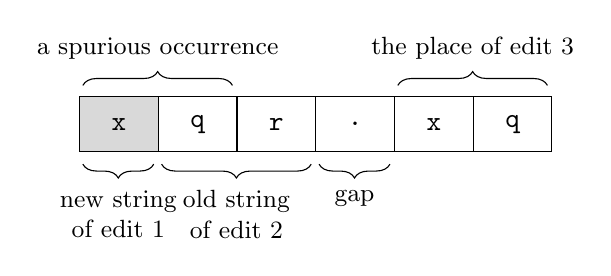
\begin{tikzpicture}[x=1cm,y=1cm,letter/.style={draw,minimum width=1cm,minimum height=0.7cm,font=\ttfamily,inner sep=0pt,anchor=south west}]
  \node[letter,fill=black!15] at (0,0) {x};
  \node[letter] at (1,0) {q};
  \node[letter] at (2,0) {r};
  \node[letter] at (3,0) {.};
  \node[letter] at (4,0) {x};
  \node[letter] at (5,0) {q};
  \draw[decorate,decoration={brace,amplitude=5pt}] (0.05,0.85) -- (1.95,0.85) node[midway,above=6pt,font=\small] {a spurious occurrence};
  \draw[decorate,decoration={brace,amplitude=5pt}] (4.05,0.85) -- (5.95,0.85) node[midway,above=6pt,font=\small] {the place of edit 3};
  \draw[decorate,decoration={brace,mirror,amplitude=5pt}] (0.05,-0.15) -- (0.95,-0.15) node[midway,below=6pt,font=\small,align=center] {new string\\of edit 1};
  \draw[decorate,decoration={brace,mirror,amplitude=5pt}] (1.05,-0.15) -- (2.95,-0.15) node[midway,below=6pt,font=\small,align=center] {old string\\of edit 2};
  \draw[decorate,decoration={brace,mirror,amplitude=5pt}] (3.05,-0.15) -- (3.95,-0.15) node[midway,below=6pt,font=\small] {gap};
\end{tikzpicture}
\caption{The text \str{pqr.xq} after its first edit, $\edit{p}{x}$. The old string of the third
edit, \str{xq}, occurs a second time. The occurrence touches the first edit, whose new string
it contains, and it cuts the second, whose old string it overlaps in part. It is there as long
as the first edit has been made and the second has not.}\label{fig:anatomy}
\end{figure}

\section{Finding an Order}\label{sec:orders}

\subsection{Monotone Batches}

A valid batch is \emph{monotone} on $s$ if an edit that is clean after a set of edits is
clean after every subset of it. Making more edits first can then only hurt. By
Theorem~\ref{thm:constraints} a batch is monotone if no pair of its constraints has a cut
edit. For such a batch the order can be built from its end.

\begin{quote}
\emph{From the end.} Let $R$ be the set of all edits. As long as $R$ is not empty, pick an
edit $k$ of $R$ that is clean after $R \setminus \{k\}$, put it before the edits that were
picked so far, and remove it from $R$. If there is no such edit, give up.
\end{quote}

\begin{theorem}[From the end]\label{thm:end}
Let $B$ be valid on $s$. Every order that the procedure returns works. If $B$ is monotone and
some order works, the procedure returns an order, whichever edits it picks.
\end{theorem}

\begin{proof}
In the order that is returned, the edits before an edit $k$ are the edits that were in $R$
with $k$ when it was picked, and $k$ is clean after them. So the order works, by
Theorem~\ref{thm:one}.

Let $B$ be monotone, let some order work, and let $R$ be the set that the procedure has
reached. Take the edit $k$ of $R$ that comes last in the working order among the edits of
$R$. It is clean after the set of edits before it in that order, and this set contains $R
\setminus \{k\}$. As the batch is monotone, $k$ is clean after $R \setminus \{k\}$. So the
procedure can pick, and it never gives up.
\end{proof}

The procedure asks at most $n^2$ times whether a string occurs once in a text, and each
question is answered in time linear in that text \citep{KMP1977}. The constraints of a
monotone batch say that an edit comes before at least one edit of each of several sets.
Read backwards in time, these are AND/OR precedence constraints, for which the same greedy
argument is known from scheduling \citep{Mohring2004}.

\subsection{Batches Whose Places Are Apart}

Let $\ell$ be the length of the longest old string of a batch. The batch is \emph{separated}
on $s$ if any two of its places have at least $\ell - 1$ letters of the snapshot between
them. Say that edit $j$ \emph{spoils} edit $k$ if $u_k$ occurs more than once after $j$ alone
has been made.

\begin{theorem}[Separated batches]\label{thm:separated}
Let $B$ be valid and separated on $s$. An order works exactly if every edit comes before every
edit that spoils it. So some order works exactly if the relation of spoiling has no cycle,
and the orders that work are its topological orders, reversed.
\end{theorem}

\begin{proof}
A spurious occurrence of $u_k$ has at most $\ell$ letters. If it touched two edits, or
touched one and overlapped the old string of another, be it that of $k$ itself, it would
contain a letter of each, or a letter on the far side
of each deletion, and all the letters between the two places. These are at least $\ell + 1$
letters. So every spurious occurrence touches exactly one edit and cuts none, and the
constraints of $k$ are the pairs $(\{j\}, \emptyset)$ for the edits $j$ that spoil $k$. The
claim is then Theorem~\ref{thm:constraints} with Theorem~\ref{thm:one}.
\end{proof}

The swap of Section~\ref{sec:accidents} is separated, and each of its edits spoils the other.
That cycle is the reason why it has no order. The first accident is one arrow. Whether one
edit spoils another is decided by a string search around the place of the first, so the graph
costs $n^2$ short searches. A model can apply the rule without any search in most cases:
\emph{an edit whose new string contains the old string of another edit goes after that
edit.}

\subsection{The General Case}

Batches whose places are close can fail to be monotone, and then the procedure can take a
wrong turn. \claim{stuck}{In the batch on \str{pqr.xq} of Section~\ref{sec:anatomy} two
orders work, both with the third edit last. The second edit is clean after the other two, so
the procedure may pick it as the last, and then it gives up; if it picks the third edit, it
succeeds.} The batch is not monotone: the third edit is clean after the other two and not
after the first alone.

This is no weakness of the procedure.

\begin{theorem}[Hardness]\label{thm:hard}
It is NP-complete to decide whether a valid batch has an order that works.
\end{theorem}

\begin{proof}
The problem is in NP, because an order can be guessed and run. For the hardness we reduce from
an ordering problem of \citet{Guttmann2006}. An instance is a finite set, a collection of
pairs $(p, q)$ of its elements, and a collection of triples $(a, k, b)$ of distinct elements,
such that no element is in two triples. The question is whether the set has a total order in
which $p$ comes before $q$ for every pair, and in which for no triple $a$ comes before $k$
and $k$ before $b$. Among the constraints on triples that the authors classify, this is the
one that forbids one of the six orders of a triple, and it is NP-complete also for disjoint
triples; the report version has the proof \citep{Guttmann2005}.

Given an instance, we build a text and a batch with one edit for every element. Below, a
\emph{fresh} letter is one that is used nowhere else.
\begin{itemize}
\item \emph{Old strings.} For every triple $t = (a, k, b)$ take fresh letters $\chi_t$,
  $\beta_t$ and $\beta'_t$. The old string of $b$ is $\beta_t\beta'_t$, and the old string of
  $k$ is $\chi_t\beta_t$. Every other element has an old string of two fresh letters.
\item \emph{New strings.} The new string of an element $q$ begins with a fresh letter. Then,
  for every pair $(p, q)$, it has a copy of the old string of $p$ and a fresh letter. If $q$
  is the first element $a$ of a triple $t$, it ends with $\chi_t$.
\item \emph{The snapshot.} It has every old string once, with fresh letters between them,
  except that for every triple the old string of $a$ is followed at once by the old string of
  $b$.
\end{itemize}
The batch is valid. Fresh letters stand between everything, so in a text $\Par(S, s)$ an old
string can occur only in three ways: as its place, as a copy inside a new string, and, for
the string $\chi_t\beta_t$ of a triple, where the new string of $a$ ends and the old string
of $b$ begins. A copy stays for good, because no place lies inside a new string. So the edit
of an element $p$ is refused exactly if some $q$ with a pair $(p, q)$ has been made, and the
edit of the middle element $k$ of a triple is refused moreover exactly while $a$ has been
made and $b$ has not. By Theorem~\ref{thm:one}, an order of the edits works exactly if it is
an order that the instance asks for.
\end{proof}

The text of the proof uses as many letters as it needs. For a batch of a few edits the
hardness does no harm. A set of edits is \emph{reachable} if its edits can be made in some
order, a reachable set stays reachable when an edit is added that is clean after it, and the
search over the reachable sets decides whether an order exists. It looks at no more than
$2^n$ sets.

\subsection{When No Order Works}

A batch without an order can be repaired in two ways, a cheap one that does not always
succeed and a dear one that does. The cheap one is what a model does when an edit is refused:
it gives the edit more context.

\begin{proposition}[Context]\label{prop:context}
Let $B$ be valid on $s$, let $x$ and $y$ be the letters of the gaps that stand directly
before and after the place of an edit $u_k \mapsto v_k$, as many as one likes, and let $B'$
be $B$ with that edit replaced by $x\,u_k\,y \mapsto x\,v_k\,y$. Then $B'$ is valid on $s$
and has the same parallel meaning, and every order that works for $B$ works for $B'$.
\end{proposition}

\begin{proof}
The string $x\,u_k\,y$ occurs in $s$ where it stands and nowhere else, because each of its
occurrences contains one of $u_k$. Its place overlaps no other place, because $x$ and $y$
come from gaps. The same letters are replaced by the same letters, so the texts $\Par(S, s)$
are the same for both batches, and the other edits are clean after the same sets. A spurious
occurrence of the longer string contains a spurious occurrence of $u_k$, because the letters
of $x$ and $y$ are never replaced and stand around the segment of $k$ in every text. So the
longer edit is clean wherever the shorter one is, and Theorem~\ref{thm:one} gives the claim.
\end{proof}

Context can only add orders, and two neighbours must not take the same letter of the gap
between them. \claim{swap-context}{For the swap one letter is enough. If the second edit
takes the blank before \str{hi} into both of its strings, the first edit no longer spoils
it, and the order in which the first edit is made first works.} Context fails where there is
no gap to take it from, and then edits have to be merged.

\begin{proposition}[Merging]\label{prop:merge}
Let $B$ be valid on $s$, and let $j$ and $k$ be two of its edits with no other place between
theirs, $I_j$ before $I_k$, and with the gap $g$ between the two places. Replace the two
edits by the one edit that turns $u_j\,g\,u_k$ into $v_j\,g\,v_k$. The new batch is valid on
$s$ and has the same parallel meaning. Merging all edits in this way gives one edit, and it
applies to $s$.
\end{proposition}

\begin{proof}
The string $u_j\,g\,u_k$ occurs in $s$ where the two places and the gap stand. It occurs
nowhere else, because each of its occurrences contains one of $u_j$. Its place is the union
of the two places and the gap, which no other place overlaps. Replacing it by $v_j\,g\,v_k$
replaces the two places and leaves the gap.
\end{proof}

For the swap the merged edit turns \str{lo = 1; hi} into \str{hi = 1; lo}. The price is the
gap, which the model has to write twice. A harness that implements the parallel meaning
directly asks for neither repair.

\section{A Snapshot That Is No Longer Current}\label{sec:stale}

So far all edits of a batch were written for the same text. Now let an author read a text
$s$ and write one edit $e = u \mapsto v$, which applies to $s$ at the place $I$. Before the
edit arrives, the text changes: another agent, or the user, makes a batch $A$ that is valid
on $s$, and the text is now $t = \Par(A, s)$. Every change of a text can be written as such a
batch, as a comparison of the two texts shows \citep{Myers1986}. What should the harness do
with $e$?

The author looked at $s$. If the place $I$ is disjoint from the places of $A$, what the
author meant is clear: the batch $A$ and the edit $e$ together, $\Par(A \cup \{e\}, s)$. If
$I$ overlaps a place of $A$, the letters that the author wanted to replace have been
replaced already, and the edit has no meaning that both authors would accept. That is a
conflict in the usual sense.

\begin{theorem}[Old snapshots]\label{thm:stale}
Let $A$ be valid on $s$, let $e = u \mapsto v$ apply to $s$ at the place $I$, and let $t =
\Par(A, s)$.
\begin{enumerate}
\item If $I$ is disjoint from the places of $A$, then $e$ applies to $t$ exactly if $u$ has
  no spurious occurrence in $t$, and the result is then $\Par(A \cup \{e\}, s)$.
\item If $I$ overlaps a place of $A$ and $e$ applies to $t$, then the occurrence that it
  replaces touches an edit of $A$: it contains a letter that $A$ wrote, or it reaches across
  a place where $A$ deleted.
\item If $I$ is disjoint from the places of $A$, replacing the letters of $I$ where they now
  stand in $t$ gives $\Par(A \cup \{e\}, s)$, whether $u$ occurs once in $t$ or not.
\end{enumerate}
\end{theorem}

\begin{proof}
Part~1 is Theorem~\ref{thm:one} for the batch $A \cup \{e\}$, which is valid on $s$, in an
order with $e$ last. Part~3 is the definition of the parallel meaning. For part~2, an
occurrence of $u$ in $t$ that touches no edit of $A$ lies in one gap of $s$ and is an
occurrence of $u$ in $s$, as in Lemma~\ref{lem:anatomy}. The only one is $I$, which does not
lie in a gap.
\end{proof}

Part~2 is the dangerous case. \claim{wrong-place}{A file has one function, which ends in
\str{return total}, and an author writes an edit that turns this line into \str{return total
+ tax}. Meanwhile the function is rewritten to return something else, and a second function
is added that ends in \str{return total}. The old string occurs exactly once in the file as
it is now, in the second function, and a harness that checks only this makes the edit there.}
The author never saw that function.

A harness has four rules to choose from. Table~\ref{tab:stale} compares them.
\begin{itemize}
\item \emph{Refuse a changed text.} The edit is refused if the text is not the one that its
  author read. This is safe and loses every edit that could have been made.
\item \emph{Once now.} The edit is made if its old string occurs once in the text as it is
  now. Claude Code documents this rule for a file that changed after it was read
  \citep{claudecodetools}. By part~1 it does what the author meant whenever the place was not
  changed. By part~2 it can make the edit in changed text when the place was changed.
\item \emph{Once now, at a place that was not changed.} The harness also remembers which
  stretches of the text changed since the author read it, and refuses if the occurrence
  touches one of them. This rule makes only edits that mean what their authors meant.
\item \emph{Carry the place.} The harness finds the place in the snapshot and carries it
  through the changes, as operational transformation does with positions
  \citep{Ellis1989,Sun1998}. By part~3 this makes every edit whose place was not changed,
  also those that the changes spoiled from a distance, and no other.
\end{itemize}
The last two rules need the snapshot, or a record of what changed since it was taken. That is
a list of stretches for every reader and costs little.

\section{Experiments}\label{sec:experiments}

The script \texttt{edits.py} implements Sections~\ref{sec:batches} to~\ref{sec:stale}. It
trusts three small functions, which find the occurrences of a string, make one edit as a
harness does, and make a list of edits in an order. Everything else is compared with them. It
needs nothing but Python, and \texttt{make -C artifact check} runs it and compares its output
with the numbers in this paper.

\paragraph{Every pair of short edits.} The script takes every text of up to six letters over
\str{a} and \str{b}, \exPairTexts{} texts, and every pair of edits whose old strings have one
or two letters and whose new strings have at most two. \claim{pairs}{In \exPairs{} cases both
old strings occur once in the text. In \exPairValid{} of them the places are disjoint: both
orders work for \exPairBoth{}, one order for \exPairOne{}, and none for \exPairNeither{}, and
every order that works gives the parallel meaning. In the other \exPairOverlap{} the places
overlap, and for \exPairDiffer{} of these both orders work and give two different texts.} The
smallest such case is the text \str{ab} with the edits $\edit{a}{aa}$ and $\edit{ab}{ba}$,
which give \str{aba} in one order and \str{baa} in the other. Texts over two letters are an
extreme, and the shares mean nothing for real files. What the count shows is that each of the
outcomes of Section~\ref{sec:accidents} is common once strings repeat.

\paragraph{Random batches.} The script draws \exBatches{} valid batches of two to five edits
on random texts over two to four letters. Old strings have one to three letters and new ones
at most three. For every batch it runs every order, \exOrders{} orders in all.
\claim{one-meaning}{An order works exactly if every edit is clean after the edits before it,
and every order that works gives the parallel meaning, as Theorem~\ref{thm:one} says. Over
all edits and all sets of other edits, the texts have \exWindows{} spurious occurrences. Each
touches an edit that was made, none contains an old string whole, and \exCutting{} of them cut one or two old strings, as
Lemma~\ref{lem:anatomy} says. The constraints of Theorem~\ref{thm:constraints} say for every
edit and every set of other edits whether the edit is clean.}

\begin{table}
\caption{Random valid batches by their number of edits: the percentage for which every
order works, some but not every order, and no order; the percentage that are not monotone;
the number for which the procedure of Theorem~\ref{thm:end} gives up, with some way of
picking, although an order works; and the percentage that are separated.}\label{tab:orders}
\begin{tabular}{rr@{\qquad}rrr@{\qquad}rr@{\qquad}r}
\toprule
 & & \multicolumn{3}{c}{orders that work} & not & & \\
edits & batches & every & some & none & monotone & gives up & separated \\
\midrule
\rows{orders}
\bottomrule
\end{tabular}
\end{table}

\paragraph{Orders.} Table~\ref{tab:orders} shows how the batches fare. \claim{orders}{The
share of batches for which every order works falls with every further edit, from
\exEveryTwo{} percent for two edits to \exEveryFive{} percent for five. Over all batches,
\exSome{} percent work in some orders and not in others, and \exNoOrder{} percent work in
none. The search over reachable sets finds an order exactly if one works. The procedure from
the end returns only orders that work, and for every monotone batch that has an order it
returns one, with each of three ways of picking. Of the batches, \exHard{} are not monotone,
and for \exStuck{} of these the procedure gives up with some way of picking although an order
works. For the \exApart{} separated batches the orders that work are exactly those of
Theorem~\ref{thm:separated}. Merging two neighbours keeps the batch valid and its meaning,
and the batch merged into one edit applies.} The merged edit has an old string \exMergeFactor{}
times as long as the old strings of the batch together. On these short texts the gaps are
short, and in a real file the factor is the distance between the first and the last place.

\paragraph{Repair by context.} \claim{context}{In every batch the script gives one edit, drawn at
random, some context from the gaps beside it. The meaning stays, and no order is lost. Of the \exNoOrderCount{} batches with no
order, one letter of context gives an order to \exRepairOne{}, two letters to \exRepairTwo{},
and three or four to \exRepairMore{}. The other \exRepairNone{} have no order with four
letters, and need more context or a merge.} So the repair that models already use is usually
enough, and the theory says why it is safe: it changes no text and can only remove
constraints.

\paragraph{The hard problem.} \claim{hard}{For \exHardInstances{} random instances of the ordering
problem of Theorem~\ref{thm:hard}, with three to six elements, the script builds the batch of
the proof and runs every order, \exHardOrders{} in all. An order of the elements does what the
pairs and triples ask exactly if the same order of the edits works. Of the instances,
\exHardSolvable{} have such an order.}

\paragraph{Old snapshots.} The script draws \exStaleTrials{} cases of a snapshot, a valid
batch of one to three edits that is made, and one further edit that applies to the snapshot.
Table~\ref{tab:stale} counts what the four rules do.

\begin{table}
\caption{Four rules for an edit that was written for a text which has changed since: how
many edits each rule makes, how many of those are not what the author meant, and how many
edits it refuses that had a meaning.}\label{tab:stale}
\begin{tabular}{lrrr}
\toprule
rule & makes & not as meant & refuses in vain \\
\midrule
\rows{stale}
\bottomrule
\end{tabular}
\end{table}

\claim{stale}{The place of the edit is kept in \exStaleKept{} cases and changed in
\exStaleChanged{}. When it is kept, the edit is made as its author meant or refused, as
part~1 of Theorem~\ref{thm:stale} says, and it is refused in \exStaleRefused{} cases, which
is \exStaleRefusedShare{} percent. When the place is changed, the old string still occurs
once in \exStaleWrong{} cases, \exStaleWrongShare{} percent, and each time the occurrence
touches what was changed, as part~2 says.} These shares come from texts over a few letters,
in which a string of three letters is easily found again. In a real file an old string is a
line or several, and both shares are far smaller. The case of part~2 needs no small alphabet,
though, as the example of Section~\ref{sec:stale} shows. It needs a line that is common
enough to stand in two functions.

\paragraph{Planted mistakes.} A check that never fails checks nothing. The script has
\exMutants{} switches, each of which plants one mistake in an analysis: a parallel meaning
that does not move the places; a batch with overlapping places that counts as valid;
cleanness judged in the snapshot and not in the text that the earlier edits left; a deletion
that touches nothing; constraints without the edits that must not yet be made; an order built
from the front; a batch that counts as separated when it is not; the graph with its arrows
reversed; a reduction in which the two places of a triple stand apart; and the third rule for
old snapshots without its memory. \claim{all-noticed}{Each
of them is noticed by a comparison that fails.}

\section{Related Work}\label{sec:related}

\paragraph{Theories of patches.} The theory of patches behind Darcs asks when two changes
commute, and it has been given categorical and homotopical accounts
\citep{Mimram2013,Angiuli2014}. A patch there names lines by their position, and two patches
that touch different lines always commute. The edits of this paper name their place by its
content. That makes the precondition a property of the whole text, and two edits on
different lines can fail to commute. Theorem~\ref{thm:one} is a commutation result of the
kind those theories have, and Sections~\ref{sec:anatomy} and~\ref{sec:orders} are about what
they do not need: the order in which preconditions hold.

\paragraph{Merging.} Three-way merging aligns two changed texts with their common ancestor
and reports a conflict where changed regions overlap; \citet{Khanna2007} give its
properties, and \citet{Mens2002} surveys what lies beyond text. Our valid batches are the
conflict-free case. The spoiling of an edit from a distance has no counterpart in a merge,
which never searches for a string. An earlier paper of this collection merges the work of
several agents by replaying what each of them read \citep{tpp9}; this paper is about one
file and the tool with which the writes are made.

\paragraph{Concurrent editing.} Operational transformation carries the position of an
operation through the operations that were made in the meantime \citep{Ellis1989,Sun1998},
and replicated data types give every letter an identity that survives edits
\citep{Shapiro2011}. The fourth rule of Section~\ref{sec:stale} is operational transformation
for one kind of operation. What this paper adds is the comparison with the rule that
harnesses use, the search for the string in the current text, and the theorem that says
exactly when the two agree.

\paragraph{Rewriting.} An edit is a rule of a string-rewriting system \citep{BookOtto1993}
with a side condition, that the left side occurs once, and it is used once. Commutation of
rewrite steps at disjoint positions is the elementary case of the theory of confluence
\citep{Huet1980}. The side condition is what makes our steps interfere at a distance, and it
is the reason why disjoint steps commute only in the weak sense of Theorem~\ref{thm:one}:
either order gives the same text, if it gives one.

\paragraph{Ordering under constraints.} The constraints of a monotone batch are AND/OR
precedence constraints \citep{Mohring2004}. Those of a general batch forbid that an edit
stands between two others in one direction. That an element must stand between two others is
the classical hard constraint on orders \citep{Opatrny1979}, and \citet{Guttmann2006}
classify every constraint on triples. The one that a batch expresses is among the hard ones,
and it stays hard when no element is in two triples. That matters here, because an edit has
one place and can be the neighbour of only two others.

\section{Limits}\label{sec:limits}

\paragraph{Strings, not syntax.} An edit here is a pair of strings, and a text is a string.
Whether the edited file still parses, or means what was meant, is outside the paper. Two
edits that commute as strings can break each other as code.

\paragraph{One tool.} Tools for editing also replace every occurrence of a string, write a
whole file, or insert at a line. We treat only the edit that requires one occurrence. For
the edit that replaces all occurrences the analysis would be another one, because such an
edit is never refused for a second occurrence.

\paragraph{Many letters.} The batches in the proof of Theorem~\ref{thm:hard} use more letters
the more elements the instance has. We have not shown that the problem stays hard over a
fixed alphabet. We also have no bound for batches of the kind that agents write, with long
old strings and few edits, other than the search.

\paragraph{No real batches.} The experiments use random texts over few letters, where
strings repeat far more often than in code. They test the theorems and say nothing about
how often an agent's batch fails in practice. We have not measured that.

\paragraph{Proofs on paper.} The proofs are short, and none has been checked by a machine.
The script tests their statements on small cases, against every order.

\section{Conclusion}

The edit that names its place by content is a good interface for a model and a subtle one for
a harness. Its precondition can be broken from anywhere in the file, so a batch of edits is
not a set unless the harness makes it one. It can. If the harness finds all places in the
snapshot that the edits were written for and replaces them at once, no order matters, a swap
needs no temporary name, and an edit for an old snapshot is made exactly when its place is
still there. A harness that makes edits one at a time can at least order them, from the end,
and say why when no order exists. The one thing that it should not do is to take the fact
that a string occurs once as proof that it is the string that the author saw.

\bibliographystyle{ACM-Reference-Format}
\bibliography{refs}

\end{document}
